\documentclass[a4paper,12pt,oneside,openany,table,xcdraw]{article}

\usepackage{setspace}
\usepackage{multirow}
\usepackage{hyperref}
\usepackage{caption}
\usepackage{indentfirst}

\usepackage[brazilian]{babel}
\usepackage[utf8x]{inputenc}
\usepackage{amsmath, graphicx, subfig, enumerate}
\usepackage{float, verbatim}
\usepackage[colorinlistoftodos]{todonotes}
\usepackage{makeidx} % Para o sumário
\usepackage{geometry}

\graphicspath{{img/}}
\geometry{a4paper, hmargin={3cm, 3cm}, vmargin={3cm, 2cm} }
\setlength{\parindent}{1.0cm}
\captionsetup{font=small}

\begin{document}
\newcommand{\thedepartment}{Faculdade de Engenharia Elétrica}
\newcommand{\thecourse}{FEELT}
\newcommand{\thetitle}{CIRCUITOS TRIFÁSICOS DESEQUILIBRADOS}
\newcommand{\thetype}{Relatório da Disciplina de Experimental de Circuitos Elétricos II}
\newcommand{\theproftitle}{Bacharel em Engenharia Elétrica}
\newcommand{\thestudent}{Lesly Viviane Montúfar Berrios\\
\centering11811ETE001}
\newcommand{\theadvisor}{Prof. Wellington Maycon Santos Bernardes}
\newcommand{\thecity}{Uberlândia}

\thispagestyle{empty}\newcommand*{\themonth}{\ifthenelse{\the\month < 2}{Janeiro }
                  {\ifthenelse{\the\month < 3}{Fevereiro }
                  {\ifthenelse{\the\month < 4}{Março }
                  {\ifthenelse{\the\month < 5}{Abril }
                  {\ifthenelse{\the\month < 6}{Maio }
                  {\ifthenelse{\the\month < 7}{Junho }
                  {\ifthenelse{\the\month < 8}{Julho }
                  {\ifthenelse{\the\month < 9}{Agosto }
                  {\ifthenelse{\the\month < 10}{Setembro }
                  {\ifthenelse{\the\month < 11}{Outubro }
                  {\ifthenelse{\the\month < 12}{Novembro }{Dezembro }}}}}}}}}}}}
                  
\begin{titlepage}
\begin{center}

	\vspace{-0.5cm}

  \begin{figure}[hbt!]
		\begin{center}
		   
\includegraphics[width=2.8cm]{ufu-logo.png}
		\end{center}
	\end{figure}
 	%\vspace{-4cm}

%\begin{doublespacing}

  \Large{\textbf{Universidade Federal de Uberlândia}}\\
  \large{\thedepartment}\\
  \large{\thecourse}\\


\vspace{5.8cm}
  \par
  \large\textbf{\thetitle}
\vspace{5.8cm} 

%\end{doublespacing}
  \par
  \thetype\\
  por\\
  %\hspace{2cm}\large{}\\

\vspace{0.8cm}
\par
  \normalsize{\thestudent}\\ [2cm]
  \theadvisor

\par\vfill
  \thecity, \themonth / \the\year

\end{center}

\end{titlepage}

%% Comeca o documento !

\onehalfspacing
\tableofcontents % sumário
\newpage

\section{Objetivos} % 2,5%
Pretende-se investigar-se experimentalmente acerca do efeito da presença do fio neutro em circuitos trifásicos desequilibrados, ligados em estrela.

\section{Introdução teórica} % 5%

Um sistema trifásico equilibrado é o ideal para geração, transmissão e distribuição de energia elétrica em corrente alternada. O uso de tensões e correntes trifásicas igualmente defasadas permite uma transferência de potência de forma igualitária e evita sobrecargas na rede. Entretanto, o desequilíbrio em cirucitos polifásicos é comum e podem ocorrer devido a prensença de cargas trifásicas desequílibradas, distribuição de cargas monofásicas sem planejamento e pela variação nos ciclos de demanda de cada fase, como observa-se na Figura \ref{intro:fig1}.

\vspace{0.3cm}
\begin{figure}[H]
\centering
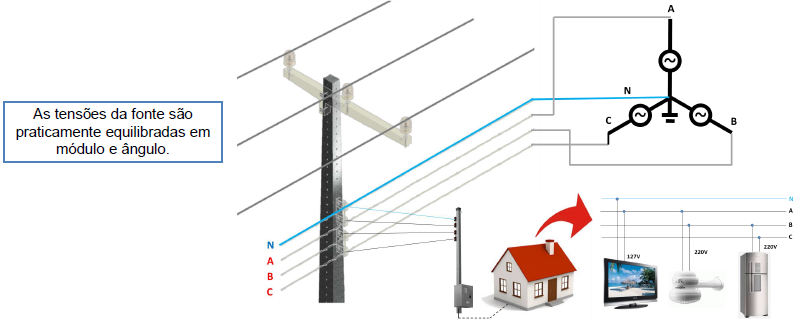
\includegraphics[width=13cm]{DISTRIBUICAO-DESUNIFORME}
\caption{Distribuição desuniforme de cargas entre as fases \cite{PH}.}
\label{intro:fig1}
\end{figure}
\vspace{0.3cm}

Nesse contexto, é de interesse estudar circuitos elétricos desequilibrados, com o intuito de verficar os efeitos do deslocamento do neutro na rede elétrica. 

\vspace{0.2cm}
\subsection{Método dos 3 Wattímetros}
O método dos 3 wattímetros, no qual é conectado um wattímetro por fase, é pouco comum, a menos que se deseje as potências de cada fase. É aplicável em circuitos onde o fator de potência varia continuamente como, por exemplo, no caso da obtenção das características de um motor síncrono, que graças a seu fator de potência elevado e variável são usados na correção de fator de
potência e precisam de uma fonte de corrente contínua ou retificada para sua excitação, além de
exigirem um complexo equipamento de controle. 

Para circuitos elétricos a 4 Fios ($\mathrm{Y}$ com neutro) necessariamente, deve-se utilizar esse método, como no circuito da primeira montagem desse experimento (Figura \ref{m1:esquema}). A medição de potência de cada wattímetro por fase referente a um ponto $\mathbf{P}$, como mostrado na Figura \ref{intro:fig2}. Ainda é possível provar a indepência da medição de cada wattímetro com o ponto $\mathbf{P}$, que pode ligar-se a qualquer uma das fases caso não haja neutro (sistema a 3 fios). Assim, o wattímetro correspondente à fase ligada ao ponto P será desnecessário para a medição da potência trifásica pois medirá com $V_L=0V$, recaindo se, portanto, no método dos dois wattímetros

\vspace{0.3cm}
\begin{figure}[H]
\centering
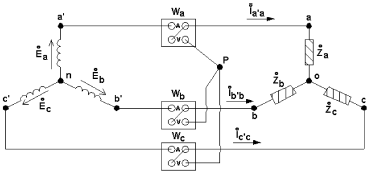
\includegraphics[width=13cm]{3Watt}
\caption{Ligação de wattímetros no sistema trifásico \cite{PH}.}
\label{intro:fig2}
\end{figure}
\vspace{0.2cm}


\section{Preparação}
\subsection{Materiais e ferramentas} % 2,5%
\begin{enumerate}[1 -]
\item \emph{\textbf{Fonte:}}
Alimentará todo o circuito. Possui frequência de $60\ Hz$.

\item \emph{\textbf{Regulador de tensão (Varivolt):}}
Também chamado de autotransformador, permitirá obter o valor desejado de corrente a partir da regulagem correta da tensão fornecida pela fonte.

\item \emph{\textbf{Conectores:}}
Para as conexões no circuito foi utilizado majoritariamente cabos banana-banana.

\item \emph{\textbf{Medidor eletrônico KRON Mult K:}}
Possibilita encontrar a medição da potência real (P) - vatímetro, reativa (Q) e aparente (S) do circuito. Ele também possui função de cofasímetro, instrumento elétrico que mede o fator de potência (fp, $cos\theta$) ou o ângulo da impedância $\theta$ do circuito, para um circuito com a impedância $Z = Z\angle \theta$.

\item \emph{\textbf{Amperímetro analógico AC:}}
Instrumento utilizado para acompanhar visualmente o aumento da corrente.

\item \emph{\textbf{Reatores de 200 mH:}}
Foram utilizados 3, para compor a carga do circuito trifásico. Sendo $L=200mH$ e $R_L=3,8\Omega$.

\item \emph{\textbf{Resistores de $50\Omega$:}}
Foram utilizados 3, para compor a carga do circuito trifásico.

\item \emph{\textbf{Capacitores de $45,9\mu F$:}}
Foram utilizados 3, para compor a carga do circuito trifásico. Sendo $C= 45,9\mu F$. Sendo sua resistência quase nula, portanto desprezível nessa aplicação (Esquenta pouco, logo dissipa menos energia).
\end{enumerate}

\vspace{0.2cm}
\subsection{Montagem} % 2,5%

\subsubsection{Carga em estrela com neutro conectado} \label{m1:montagem}
A montagem utilizada observa-se na Figura \ref{m1:esquema}, a qual ilustra o circuito na sequência de fases ABC. Pretende-se com este circuito investigar-se acerca do efeito do neutro em circuitos trifásicos desequilibrados. Usou-se TL=0000, TC=TP=1 como configurações no medidor \emph{Kron}. Aplica-se uma tensão linha $V_L=100V$ com o auxílio do \emph{Varivolt}, em frequência de 60Hz. Ademais, a carga desequilibrada possui os seguintes parâmetro: $R=50\Omega$, $R_L=3,8\Omega$, $L=166mH$ e $C=45,9 \mu F$.

\vspace{0.2cm}
\begin{figure}[H]
\centering
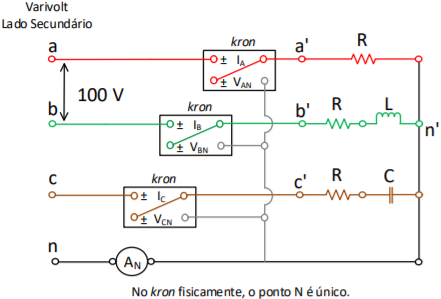
\includegraphics[width=13cm]{m1-circuito}
\caption{Circuito esquemático da montagem 1.}
\label{m1:esquema}
\end{figure}

\subsubsection{Carga em estrela com neutro isolado} \label{m2:montagem}
Com os mesmos parâmetros de impedância e tensão de entrada, porém agora com neutro isolado, mantém-se a configuração do medidor \emph{Kron}. Entretanto, nessa situação espera-se deslocamento da tensão no neutro, ou seja, $V_{n'n} \ne 0$.

\vspace{0.1cm}
\begin{figure}[H]
\centering
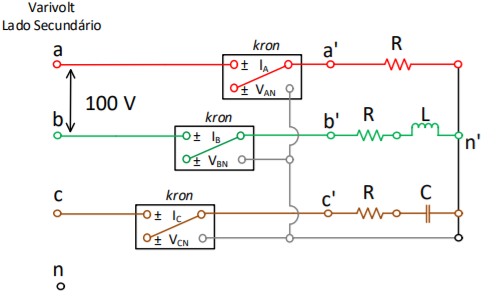
\includegraphics[width=13cm]{m2-circuito}
\caption{Circuito esquemático da montagem 2.}
\label{m2:esquema}
\end{figure}
\vspace{0.1cm}

\subsubsection{Carga em triângulo desequilibrado} \label{m3:montagem}
Agora, na conexão em triângulo e sem neutro, a configuração TL é diferente (TL=0048, $3\phi$ sem Neutro). Nessa montagem, tem-se tensão de entrada $V_{AB}=50V$, a fim de evitar-se correntes próximas ou superiores a $1,8A$ no medidor \emph{Kron}. 

\vspace{0.15cm}
\begin{figure}[H]
\centering
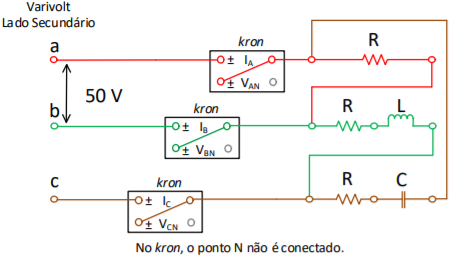
\includegraphics[width=13cm]{m3-circuito}
\caption{Circuito esquemático da montagem 3.}
\label{m3:esquema}
\end{figure}
\vspace{0.2cm}

\section{Dados Experimentais}

\subsection{Carga em estrela com neutro conectado} \label{m1:dados}
Dos dados da Tabela \ref{m1:dados:abc}, ainda tem-se $P_T = 115,5$W, $Q_T = 61,42$VAr e $S_T = 144,24$VA. Enquanto que para sequência de fases CBA (Tabela \ref{m1:dados:cba}), $P_T = 118,16$W, $Q_T = 60,7$VAr e $S_T = 155,79$VA.

\begin{table}[H]
\centering \small \def\arraystretch{1.32}
\caption{Dados experimentais da primeira montagem em sequência ABC.}
\label{m1:dados:abc}
\resizebox{\textwidth}{!}{%
\begin{tabular}{c|c|c|c|c|c|c|c|c|c|}
\cline{2-10}
                        & $V_L$ (V) & $V_F$ (V) & $I_L$ (A) & P (W) & Q (VAr) & S (VA) & FP    & $A_N$ (A)             & $V_{N'N}$  (V)        \\ \hline
\multicolumn{1}{|c|}{A} & 96,10     & 55,89     & 1,13      & 63,84 & 0,30    & 64,16  & 1     & \multirow{3}{*}{0,21} & \multirow{3}{*}{0} \\ \cline{1-8}
\multicolumn{1}{|c|}{B} & 100,07     & 56,57     & 0,62      & 22,12 & 27,68   & 35,58  & 0,625 &                       &                    \\ \cline{1-8}
\multicolumn{1}{|c|}{C} & 99,69     & 58,82     & 0,76      & 29,54 & 33,44   & 44,50  & 0,659 &                       &                    \\ \hline
\end{tabular}%
}
\end{table}

\begin{table}[H]
\centering \small \def\arraystretch{1.32}
\caption{Dados experimentais da primeira montagem em sequência CBA.}
\label{m1:dados:cba}
\resizebox{\textwidth}{!}{%
\begin{tabular}{c|c|c|c|c|c|c|c|c|c|}
\cline{2-10}
                        & $V_L$ (V) & $V_F$ (V) & $I_L$ (A) & P (W) & Q (VAr) & S (VA) & FP    & $A_N$ (A)            & $V_{N'N}$  (V)     \\ \hline
\multicolumn{1}{|c|}{A} & 100,50    & 57,60     & 1,096     & 63,25 & 0,24    & 63,51  & 1    & \multirow{3}{*}{1,6} & \multirow{3}{*}{0} \\ \cline{1-8}
\multicolumn{1}{|c|}{B} & 99,25     & 57,45     & 0,641     & 23,94 & 27,85   & 36,76  & 0,652 &                      &                    \\ \cline{1-8}
\multicolumn{1}{|c|}{C} & 100,70    & 58,34     & 0,767     & 30,57 & 32,61   & 55,52  & 0,683     &                      &                    \\ \hline
\end{tabular}%
}
\end{table}

\subsection{Carga em estrela com neutro isolado} \label{m2:dados}
Dos dados da Tabela \ref{m2:dados:abc}, ainda tem-se $P_T = 122,92$W, $Q_T = 55,16$VAr e $S_T = 149,04$VA. Enquanto que para sequência de fases CBA (Tabela \ref{m2:dados:cba}), $P_T = 125,598$W, $Q_T = 146,509$VAr e $S_T = 193,813$VA.

\begin{table}[H]
\centering \small \def\arraystretch{1.32}
\caption{Dados experimentais da segunda montagem em sequência ABC.}
\label{m2:dados:abc}
\begin{tabular}{c|c|c|c|c|c|c|c|c|}
\cline{2-9}
                        & $V_L$ (V) & $V_F$ (V) & $I_L$ (A) & P (W) & Q (VAr) & S (VA) & FP    & $V_{N'N}$ (V)      \\ \hline
\multicolumn{1}{|c|}{A} & 96,01     & 62,03     & 1,24      & 77,34 & 0,30    & 77,60  & 1     & \multirow{3}{*}{0} \\ \cline{1-8}
\multicolumn{1}{|c|}{B} & 100,6     & 54,74     & 0,59      & 20,24 & 25,60   & 32,78  & 0,621 &                    \\ \cline{1-8}
\multicolumn{1}{|c|}{C} & 99,51     & 54,98     & 0,70      & 25,34 & 29,26   & 38,66  & 0,654 &                    \\ \hline
\end{tabular}
\end{table}

\begin{table}[H]
\caption{Dados experimentais da segunda montagem em sequência CBA.}
\label{m2:dados:cba}
\centering \small \def\arraystretch{1.32}
\begin{tabular}{c|c|c|c|c|c|c|c|c|}
\cline{2-9}
                        & $V_L$ (V) & $V_F$ (V) & $I_L$ (A) & P (W) & Q (VAr) & S (VA) & FP    & $V_{N'N}$ (V)      \\ \hline
\multicolumn{1}{|c|}{A} & 100,4     & 14,18     & 0,210     & 3,968 & 0,069   & 3,963  & 1     & \multirow{3}{*}{42} \\ \cline{1-8}
\multicolumn{1}{|c|}{B} & 97,79     & 81,92     & 1,002     & 57,21 & 72,29   & 91,69  & 0,690 &                     \\ \cline{1-8}
\multicolumn{1}{|c|}{C} & 101,4     & 87,82     & 1,123     & 64,42 & 74,15   & 98,16  & 0,655 &                     \\ \hline
\end{tabular}
\end{table}

\subsection{Carga em triângulo desequilibrado} \label{m3:dados}
Dos dados da Tabela \ref{m3:dados:abc}, ainda tem-se $P_T = 88,603$W, $Q_T = 37,569$VAr e $S_T = 96,969$VA. Enquanto que para sequência de fases CBA (Tabela \ref{m3:dados:cba}), $P_T = 94$W, $Q_T = 4,303$VAr e $S_T = 91,19$VA.

\begin{table}[H]
\centering \small \def\arraystretch{1.32}
\caption{Dados experimentais da terceira montagem em sequência ABC.}
\label{m3:dados:abc}
\begin{tabular}{c|c|c|c|c|c|}
\cline{2-6}
                        & $I_L$ (A) & P (W) & Q (VAr) & S (VA) & FP    \\ \hline
\multicolumn{1}{|c|}{A} & 5,63      & 42,38 & 17,26   & 45,82  & 0,925 \\ \hline
\multicolumn{1}{|c|}{B} & 1,472     & 39,40 & 17,75   & 43,84  & 0,911 \\ \hline
\multicolumn{1}{|c|}{C} & 0,266     & 6,823 & 2,559   & 7,309  & 0,934 \\ \hline
\end{tabular}
\end{table}

\begin{table}[H]
\centering \small \def\arraystretch{1.32}
\caption{Dados experimentais da terceira montagem em sequência CBA.}
\label{m3:dados:cba}
\begin{tabular}{c|c|c|c|c|c|}
\cline{2-6}
 & $I_L$ (A) & P (W) & Q (VAr) & S (VA) & FP \\ \hline
\multicolumn{1}{|c|}{A} & 1,018 & 29,56 & 3,584 & 29,81 & 0,993 \\ \hline
\multicolumn{1}{|c|}{B} & 0,963 & 28,35 & 0,628 & 28,35 & 1 \\ \hline
\multicolumn{1}{|c|}{C} & 1,21 & 36,09 & 0,091 & 33,03 & 1 \\ \hline
\end{tabular}
\end{table}


\section{Análise sobre segurança} % 2,5%
Os óculos de segurança são Equipamentos de Proteção Individual (EPIs) e são utilizados para a proteção da área ao redor dos olhos contra qualquer tipo de detrito estranho, que possa causar irritação ou ferimentos. Também protegem contra faíscas, respingos de produtos químicos, detritos, poeira, radiação e etc \cite{safe}.
É importante a utilização desse equipamento durante os experimentos a fim de evitar qualquer dano, além de preparar o profissional para o manejo correto e seguro de qualquer equipamento.
Além disso, foi de extrema importância a presença do professor ou técnico na verificação da montagem do circuito antes de energizá-lo. Assim, reduziu-se riscos de curtos-circuitos ou sobrecarga na rede.


\section{Cálculos, análise dos resultados e questões} % (quando houver) (70%)

\subsection{Análise teórica do circuito}
Como o circuito é desequilibrado, a análise deve ser feita fase por fase. No entanto, há uma certeza: as tensões da fonte são equilibradas em módulo e ângulo. Assim, sabendo-se que $\mathrm{V_{L} =V_{F}\sqrt{3} \ \angle 30^{\circ }}$, tem-se os seguintes dados:

\vspace{-0.4cm}
\begin{equation*}
\begin{array}{ c c c }
\mathrm{\begin{bmatrix}
E_{AB}\\
E_{BC}\\
E_{CA}
\end{bmatrix} =100V\ \begin{bmatrix}
1\\
\alpha ^{2}\\
\alpha 
\end{bmatrix}} & \quad \text{e} \quad \  & \mathrm{\begin{bmatrix}
E_{AN}\\
E_{BN}\\
E_{CN}
\end{bmatrix} =57,74V\ \angle -30^{\circ } \begin{bmatrix}
1\\
\alpha ^{2}\\
\alpha 
\end{bmatrix}}
\end{array}
\end{equation*}

\vspace{0.2cm}
\subsubsection{Carga em estrela com neutro conectado} \label{m1:teoria}
Primeiramente, é possível descrever as impedâncias como abaixo:

\vspace{-0.5cm}
\begin{equation*}
\begin{aligned}
\begin{cases}
Z_{A} =50\ [ \Omega ]\\
Z_{B} =53,8+j\ 62,58\ [ \Omega ]\\
Z_{C} =50-j\ 57,79\ [ \Omega ]
\end{cases} & \quad \text{e também} \quad  & \begin{cases}
Y_{A} =0,02\ [ S]\\
Y_{B} =0,0122\ \angle -49,31\ [ S]\\
Y_{C} =0,0131\ \angle \ 49,13\ [ S]
\end{cases}
\end{aligned}
\end{equation*}

Como os neutros da fonte e da carga estão conectados, não há deslocamento de neutro, $V_{n'n}=0$. Portanto, a tensão na carga é a mesma da fonte, como consequência da presença do neutro.

\subsubsection{Carga em estrela com neutro isolado} \label{m2:teoria}

\subsubsection{Carga em triângulo desequilibrado} \label{m3:teoria}

\subsection{Análise comparativa: experimento \emph{vs.} teoria}
\subsubsection{Sobre a presença do neutro no circuito desequilibrado}
% - Como se manifestou o desequilíbrio do sistema com a presença do fio neutro?
Como visto na análise teorica e experimental, a ligação do neutro da fonte com o da carga provocou $V_{n'n}=0$, fazendo com que a tensão fornecida pela fonte seja completamente recaída sobre a carga. Entretanto, o fio neutro tbm funciona como fuga para a corrente resultante, sendo $I_N=I_A+I_B+I_C$, já que no circuito desequilibrado as correntes não se anularão. 

\subsubsection{Sobre a ausência do neutro no circuito desequilibrado}
% - Como se manifestou o desequilíbrio do sistema com a ausência do fio neutro?
Na ausência do fio neutro a corrente resultante da soma das correntes de linha $I_A$, $I_B$ e $I_C$ não tem como fugir pelo neutro, além disso manisfesta-se por meio de uma diferença de potencial $V_{n'n}$, uma vez que o neutro da carga não estará mais conectado ao da fonte (referencial), que neste momento está isolado.

\subsubsection{Ilustrando as medidas de tensão e corrente na forma de fasores}
% - Usando os módulos das tensões e correntes medidas, obtenha os fasores correspondentes
% e faça um diagrama fasorial de cada caso, em ambas as sequências
A partir do resultado teórico, é interessante verficar a disposição de grandezas de tensão e corrente num diagrama fasorial, assim constatar o desequílibrio visualmente (Figura \ref{fasores}).
\vspace{0.15cm}
\begin{figure}[H]
\centering
\subfloat[]{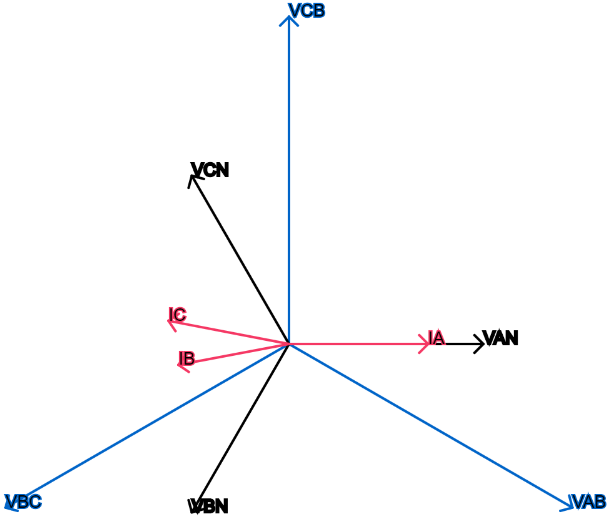
\includegraphics[width=0.5\textwidth]{m1-fasores-abc}}\hfill
\subfloat[]{\includegraphics[width=0.5\textwidth]{m1-fasores-cba}}

\subfloat[]{\includegraphics[width=0.5\textwidth]{m2-fasores-}}
\caption{Digrama fasorial das montagens 1-3 em (a)-(c).}
\label{fasores}
\end{figure}
\vspace{0.2cm}

\subsubsection{Sobre a configuração no medidor \emph{Kron}}
% - Dois tipos de ligações existentes no kron são: a) TL = 0003 (3ø com Neutro) e; b) TL = 0049
% (3ø sem Neutro). A primeira configuração poderia ser usada na seção 2.1? E a segunda
% configuração, poderia ser usada nas seções 2.2 e 2.3? Justifique as respostas.
Na Figura \ref{conf:kron} tem-se a aplicação apropriada para cada configuração TL, logo se a configuração TL=0003 tivesse sido usada na montagem 1, ou seja, em um circuito desequilibrado, não se obteria os valores de interesse, já que o medidor \emph{Kron} assume que a carga seja trifásica e procede os cálculos das grandezas trifásicas, por meio de somente os sinais de tensão e uma corrente. Assim, a impedância de uma fase qualquer é facilmente calculada pela Lei de Ohm, a qual o \emph{Kron} considerará erroneamente como a mesma impedância para as outras duas fases.

Com relação a segunda configuração (TL=0049), para as outras duas montagem, também não é possível, já que nessa configuração assume-se cargas equilibradas, assim o \emph{Kron} fará o cálculo da  terceira a partir da aritmética das outras duas obrtidas medainte, o que é erróneo, pois dado que as cargas são desenquilidadas, as corrente também deveriam ser, à tensão de linha equilibrada.  

\vspace{0.15cm}
\begin{figure}[H]
\centering
\subfloat[]{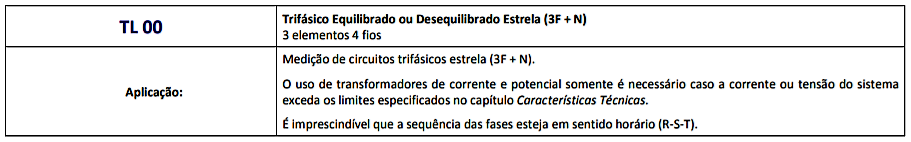
\includegraphics[width=\textwidth]{TL00}}\hfill

\subfloat[]{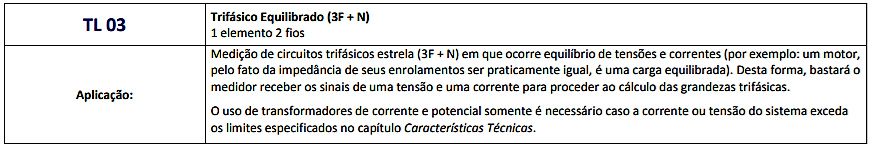
\includegraphics[width=\textwidth]{TL03}}\hfill

\subfloat[]{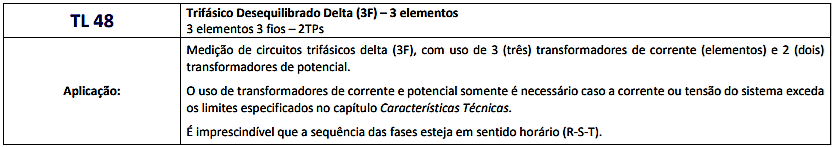
\includegraphics[width=\textwidth]{TL48}}

\subfloat[]{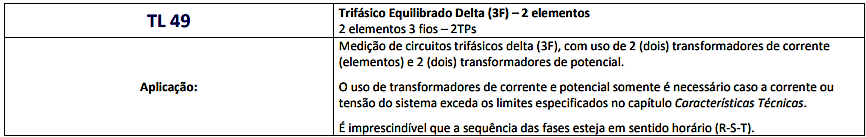
\includegraphics[width=\textwidth]{TL49}}
\caption{Informação do manual do usuário do medidor \emph{Kron} para as configurações de Tipo de Ligação (a) TL00, (b) TL03, (c) TL48 e (d) TL49 \cite{Kron}.}
\label{conf:kron}
\end{figure}
\vspace{0.2cm}


\newpage
\section{Simulação computacional} % (10%);
\subsection{Carga em estrela com neutro conectado}
\begin{figure}[H]
\centering
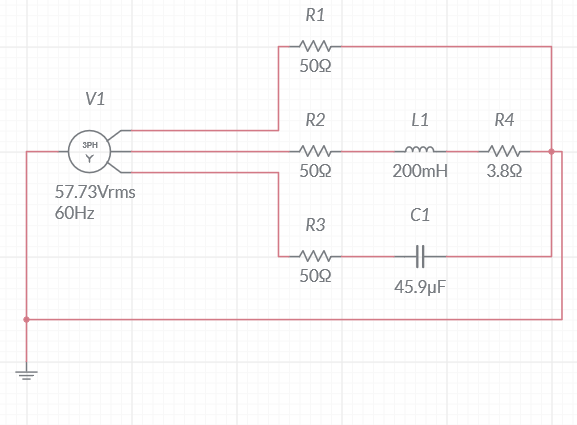
\includegraphics[width=13.5cm]{m1-esquema}
\caption{Circuito esquemático da montagem 1.}
\label{m1:esquema}
\end{figure}

\subsection{Carga em estrela com neutro isolado}

\subsection{Carga em triângulo desequilibrado}

\section{Conclusões} % (no mínimo 10 linhas) (5%);


\newpage
\begin{thebibliography}{9} 
% Introdução
\bibitem{PH}
    P. H. O. Rezende,
    "Circuitos Polifásicos Desequilibrados", 2018.

\bibitem{Kron}
    KRON Instrumentos Elétricos,
    “Mult-K 05 e Mult-K 120: Medidores de Energia e Transdutores Digitais de Grandezas Elétricas”, Kron Medidores., 2018.


\bibitem{safe}
    SafetyTrabi,
    “Óculos de segurança: Saiba quando utilizar este EPI”, SafetyTrab, 2019.
 Disponível em:
 \url{https://www.safetytrab.com.br/blog/oculos-de-seguranca/}. Acesso em: ago. 2019.


\end{thebibliography}
\end{document}
